\documentclass{beamer}
\mode<presentation>
{ \usetheme{boxes} }

\usepackage{times}
\usepackage{graphicx}
\usepackage[backend=bibtex]{biblatex}
% \addbibresourse{an_introduction_to_dogen.bib}

\title{Mesh generation from neuronal morphology files}
\author{
  \texorpdfstring
      {\href{mailto:marco.craveiro@gmail.com}{Marco Craveiro}}
      {Marco Craveiro}
}
\date{\today}

\AtBeginSection[]
{
  \begin{frame}<beamer>
    \frametitle{Outline}
    \tableofcontents[currentsection]
  \end{frame}
}

\bibliography{watertight}

\begin{document}

\begin{frame}
\titlepage
\end{frame}

\begin{frame}
\frametitle{Outline}
\begin{itemize}
\item Microscopy and Computational Neuroscience
\pause
\item SWC format
\pause
\item 3D Meshes
\pause
\item Problems with watertight mesh generation
\pause
\end{itemize}
\end{frame}

\begin{frame}
\frametitle{Microscopy and computational neuroscience}

\begin{itemize}

\item Microscopy is an important source of data on neuron morphology.
\pause
\item There are many kinds of microscopy (EM, Optical, etc.) and the
  field has evolved dramatically over the last few years.
\pause
\item The latest generation Electron Microscopes can generate
  terabytes of data at very high resolution (1 nm or higher).
\pause
\item At this resolution it is possible to see very small
  sub-structures inside of the neuron, which are important for
  morphometric work.

\end{itemize}

\end{frame}

\begin{frame}
\frametitle{Microscopy and computational neuroscience}

Example SEM (Scanning Electron Microscope) micrograph:

\begin{figure}[H]
    \centering
    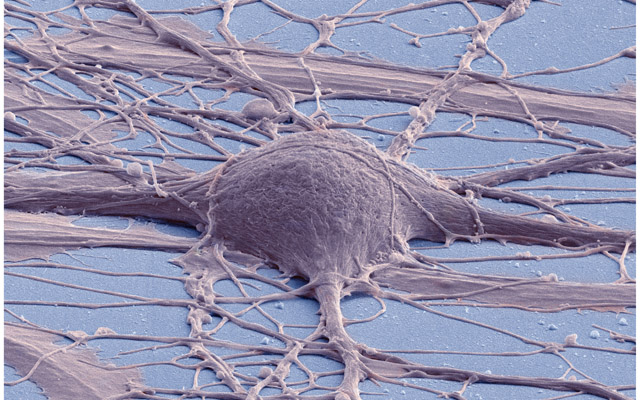
\includegraphics[scale=1.5]{../blog/images/2014_06_26_human_ipsc_derived_neuron_deerinck}
    \caption{Human neuron. Source: New Reprogramming Method Makes Better Stem Cells
      \url{http://ucsdnews.ucsd.edu/pressrelease/new_reprogramming_method_makes_better_stem_cells}.}
    \label{fig:3d_neuron}
\end{figure}

\end{frame}

\begin{frame}
\frametitle{Microscopy and computational neuroscience}

\begin{itemize}
\item The data generated by the microscopes cannot be used
  directly.
\pause
\item One must first perform recognition of the objects in the
  micrographs. This is known as \emph{segmentation} and
  \emph{reconstruction}.
\pause
\item Until recently these tasks were performed manually. Experienced
  lab technicians would identify and measure all of the structures in
  the neuron. This is a very low resolution and high-error process.
\pause
\item Recently Machine Learning has been applied to the task with
  success.
\end{itemize}

\end{frame}

\begin{frame}
\frametitle{Microscopy and computational neuroscience}

Sample micrograph from a stack. Left-hand side shows the original
micrograph; right-hand side shows the result of processing it with
machine learning.

\begin{figure}[H]
    \centering
    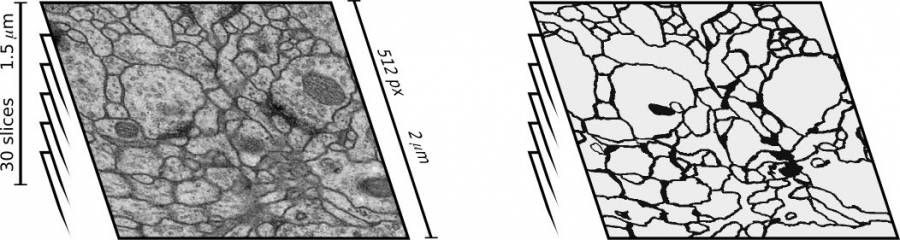
\includegraphics[scale=0.3]{../blog/images/biomed-neurons}
    \caption{Source: Deep Neural Networks Segment Neuronal Membranes in Electron Microscopy Images
      \url{http://papers.nips.cc/paper/4741-deep-neural-networks-segment-neuronal-membranes-in-electron-microscopy-images.pdf}.}
    \label{fig:stack}
\end{figure}

\end{frame}

\begin{frame}
\frametitle{Microscopy and computational neuroscience}

Reconstruction of 3D structures from a stack.

\begin{figure}[H]
    \centering
    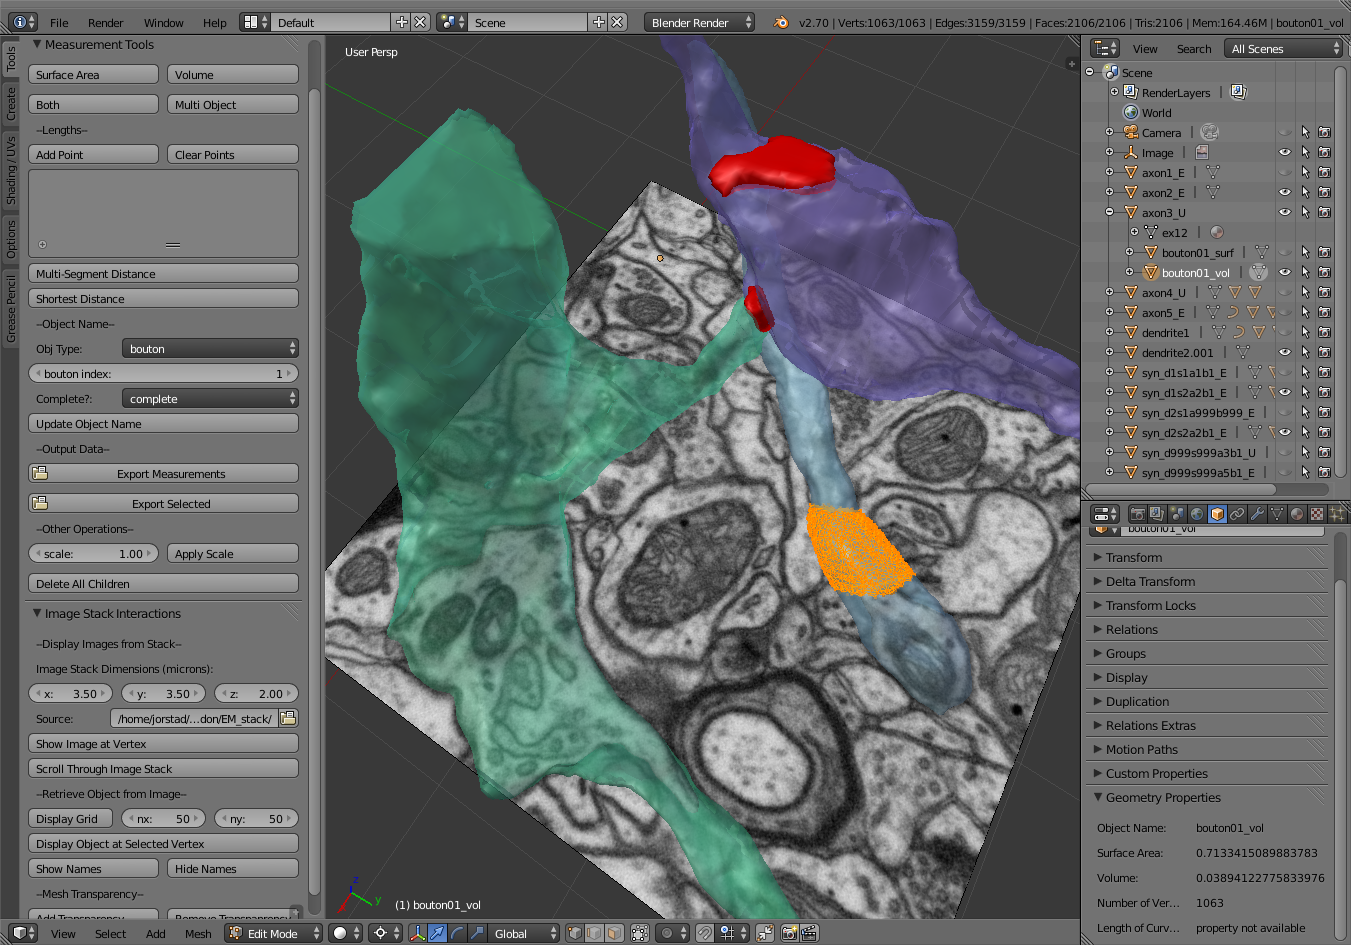
\includegraphics[scale=0.2]{../blog/images/NeuroMorph_screenshot.png}
    \caption{Source: Segmented anisotropic ssTEM dataset of neural tissue
      \url{http://figshare.com/articles/Segmented_anisotropic_ssTEM_dataset_of_neural_tissue/856713}.}
    \label{fig:3d_stack}
\end{figure}

\end{frame}

\begin{frame}
\frametitle{SWC}

\begin{itemize}

\item

\end{itemize}

\end{frame}

\begin{frame}
  \printbibliography
\end{frame}

\end{document}
